% Netzwerkanltung für die Studentenstadt Freimann
% Tex initially created by Maximilian Engelhardt <maximilian.engelhardt@stusta.mhn.de>

%\documentclass[a4paper,12pt,draft]{scrartcl}
\documentclass[a4paper,12pt]{scrartcl}

\usepackage[utf8]{inputenc}
\usepackage{ngerman}
\usepackage{eurosym}
\usepackage{tabularx}
\usepackage[pdftex,final]{graphicx}
\usepackage[top=1.5cm,bottom=2.5cm,left=1.5cm,right=1.5cm]{geometry}
%\usepackage[margin=2cm]{geometry}
\usepackage{hyperref}


\title{Wohnanlage Studentenstadt Freimann:\\
       Anleitung zum Einrichten des Internetzugangs}
%\date{\today}

\begin{document}

\maketitle

\begin{figure}[t!]
   \centering
   \vspace{-20pt}
   
\includegraphics[width=0.8\textwidth,keepaspectratio]{Bilder/StuStaNet_Logo}
   \vspace{-40pt}
\end{figure}

\section{Allgemeine Informationen zum Netzwerkanschluss}

Lesen Sie vorher die Benutzerordnung gründlich durch, die Sie mit ihrem Mietvertrag erhalten haben.
\\
\\
Sie benötigen einen Computer mit LAN-Kabelanschluss oder einen Router und ein LAN-Kabel zum Anschluss des Computers an der im Zimmer angebrachten Netzwerkdose. Diese Kabel können im Fachhandel oder auch beim StuStaNet~e.V. während der Sprechstunde (siehe weiter unten) erworben werden.
\\
\\
Jeder, der seinen Computer an das Netzwerk der Studentenstadt anschließt, ist dafür verantwortlich, dass dadurch keine anderen Rechner im Netzwerk gefährdet werden. Dazu gehört seinen Rechner vor Viren oder anderer Schadsoftware zu schützen.
Der StuStaNet~e.V. betreibt eine Schadsoftwareerkennung, die Anschlüsse bei Auffälligkeiten aufgrund von Virenbefall vorübergehend sperrt.
\begin{bfseries}
	\\Bei wiederholter Virendiagnose wird der entsprechende Anschluss dauerhaft gesperrt.
\end{bfseries}
\\
\\
In der StuSta gibt es kein zentrales WLAN in den Zimmern, allerdings kann jeder selbst einen Access Point betreiben. Der StuStaNet~e.V. verkauft auch für die StuSta passend vorkonfigurierte Router in der Sprechstunde (nur an Mitglieder).

\section{Mitgliedschaft StuStaNet~e.V.}
Es gibt zwei Möglichkeiten im Internet zu surfen. Ohne Mitgliedschaft ist der Zugang über den Proxyserver möglich. Dieser muss bei jeder Applikation eingestellt werden, falls dies unterstützt wird. Einige Software unterstützt die manuelle Proxyeinrichtung nicht, zum Beispiel Programme wie WhatsApp oder League of Legends. Damit diese funktionieren ist eine Mitgliedschaft notwendig.
\pagebreak\linebreak
Als Mitglied erfolgt der Zugang über unser NAT-Gateway. Die Konfiguration des Proxys kann dann entfallen. Außerdem stehen für Mitglieder des StuStaNet~e.V. weitere Dienste \footnote{\url{https://wiki.stusta.de/Dienste}} wie eine eigene E-Mail-Adresse, Webspace mit PHP und Datenbankunterstützung oder WLAN in Außenbereichen und Gemeinschaftseinrichtungen \footnote{\url{https://stustanet.de/de/wifi/}} zur Verfügung. 
\\
Für die Mitgliedschaft fällt eine \textbf{einmalige} Aufnahmegebühr von \EUR{20} an. Um Mitglied zu werden, registrieren Sie sich bitte unter \mbox{\url{https://reg.stustanet.de}} und werfen Sie den unterschriebenen Mitgliedsantrag in unseren Briefkasten (in Haus 10) ein. Die Adresse des Hauses lautet: Hans-Leipelt-Straße 7, 80805 München.
\\
Die Sprechstunden finden in Haus 10, Zimmer 002 (Kellergeschoss) statt. Meist Donnerstags 19:00-19:30 Uhr und zu Beginn des Semesters zusätzlich Montags 19:00-19:30 Uhr. An Feiertagen entfallen die Sprechstunden.
\\
Die genauen Zeiten sind unter \mbox{\url{https://stustanet.de}} verfügbar.

\section{Netzwerkkonfiguration}

\subsection{Zettel mit IP-Adressen des Zimmers}
\begin{minipage}{0.6\textwidth}
Als erstes wird der Zettel mit den IP-Adressen deines Zimmers benötigt.
Du solltest diesen entweder als Papierzettel beim Einzug oder als Anhang per Mail mit den Vertragsunterlagen bekommen haben. \\
Die jeweilige IP-Adresse steht auch auf einem Aufkleber auf Ihrer Anschlussbuchse. Solltest du keinen Zettel mit Netzwerkdaten bekommen haben und der Aufkleber auf der Anschlussbuchse unlesbar sein, wende dich bitte an die Hausverwaltung oder besuche unsere Sprechstunde. \\
Die Netzmaske entspricht dabei der Subnetzmaske in manchen Betriebssystemen und die entsprechende Subnetzpräfixlänge beträgt 24.
\end{minipage}
\begin{minipage}{0.4\textwidth}
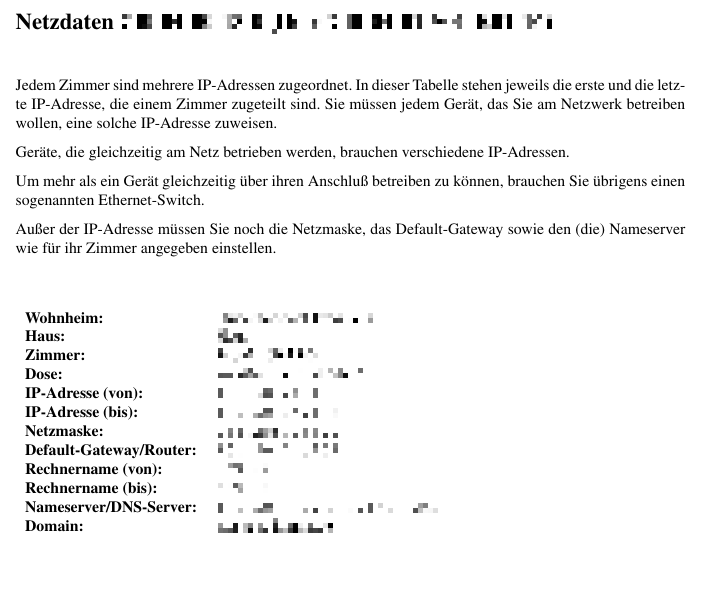
\includegraphics[width=\linewidth]{Bilder/ip_zettel}
%  \caption{Bildunterschrift}
\end{minipage}

\subsection{Verbinden eines Computers oder eines Routers mit der Netzwerkdose}

Ein Computer kann entweder direkt über ein LAN-Kabel mit der Netzwerkdose verbunden oder es kann ein Router dazwischen geschaltet werden.
Um auch WLAN verwenden zu können und für die Verwendung von mehreren Geräten ist langfristig die Nutzung eines Routers zu empfehlen. \\

Das Einrichten der Internetanbindung besteht somit aus folgenden Teilen:
\begin{itemize}
	\item Anschluss des Routers oder Computers an die Netzwerkbuchse
	\item Konfiguration der Netzwerkeinstellungen des Routers oder Betriebssystems
	\item (Nur für Nicht-Mitglieder) Eintragen des Proxyservers bzw. -skripts im Browser
\end{itemize}
Verwenden Sie ausschließlich die \emph{linke} Netzwerkbuchse.\\
Falls der Router mit den Netzwerkeinstellungen konfiguriert wird, so darf das Betriebssystem nicht auch konfiguriert werden!\\
Sollten Probleme bei der Verbindung zum Netzwerk auftreten, so ist der Besuch der Seite\\
\mbox{\url{http://selftest.stustanet.de}} hilfreich, während man mit dem nicht funktionierenden Netz verbunden ist. Hierbei wird eine Diagnose erstellt. Falls die Seite nicht erreichbar ist oder eine Fehlermeldung angezeigt wird, so ist die Netzwerkkonfiguration fehlerhaft.\\
Bei weiteren Problemen kann \mbox{\url{https://stustanet.de/de/support/}} weiterhelfen.

\subsection{Für Nicht-Mitglieder}

Bei Nicht-Mitgliedschaft beim StuStaNet e.V. muss für jedes Gerät das im Zimmer benutzt werden soll entweder das Proxyskript verwendet (empfohlen) oder manuell der Proxyserver eingestellt werden.
Nicht alle Programme unterstützen die globalen Einstellungen des Betriebssystems und unter Umständen müssen diese auch für einzelne Programme separat eingestellt werden.

%\pagebreak 

\subsection{Netzwerkeinstellungen mit den jeweiligen Proxy-Konfigurationen}
\label{subsec_settings}

Pro Anschluss stehen 8 IP-Adressen zur Verfügung. Der jeweilige Adressbereich ist auf der Netzwerkdose vermerkt oder auf dem Internetkonfigurationsblatt zu finden, das Sie mit Ihrem Mietvertrag von der Hausverwaltung erhalten haben. Sollten Sie dieses Blatt nicht mehr finden, wenden Sie sich bitte an die Hausverwaltung oder besuchen Sie unsere Sprechstunde. % \footnote{Christoph-Probst-Straße 10, Studentenstadt Freimann}.


\begin{center}
  \begin{tabularx}{\linewidth}{|lXp{.2\linewidth}|}
    \hline
    Einstellung & Wert & Beispiel \\
    \hline \hline
    IP-Adresse & \nolinkurl{10.150.xxx.yyy} - \nolinkurl{10.150.xxx.zzz}, \newline 8 Adressen stehen zur Auswahl\footnote{Auffindbar auf der Netzwerkdose im Zimmer, auf dem IP-Zettel, bei der Hausverwaltung oder in der Sprechstunde.} & \nolinkurl{10.150.243.16} – \nolinkurl{10.150.243.23} \\
    \hline
    Subnetzmaske & \nolinkurl{255.255.255.0} & \\
    \hline
    Subnetzpräfixlänge & \nolinkurl{24} & \\
    \hline
    Standardgateway & \nolinkurl{10.150.xxx.254} \newline (Die ersten drei Blöcke wie IP-Adresse, der vierte Block \nolinkurl{254}) & \nolinkurl{10.150.243.254} \\
    \hline
    DNS-Server (Nameserver) & \nolinkurl{10.150.127.2} \newline \nolinkurl{10.150.125.2} & \\
    \hline
    DNS-Suffix (Domainname) & \nolinkurl{stusta.mhn.de} & \\
    \hline
    Proxyskript & \multicolumn{2}{l|}{\nolinkurl{http://wpad.stusta.mhn.de/proxy.pac}} \\
    \hline
    Proxyserver (manuell) & \multicolumn{2}{l|}{\nolinkurl{http://proxy.stusta.mhn.de:3128}} \\
    \hline
  \end{tabularx}
\end{center}

\begin{figure}[h!]
		\centering
		\begin{minipage}[c]{0.4\linewidth}
			\centering
			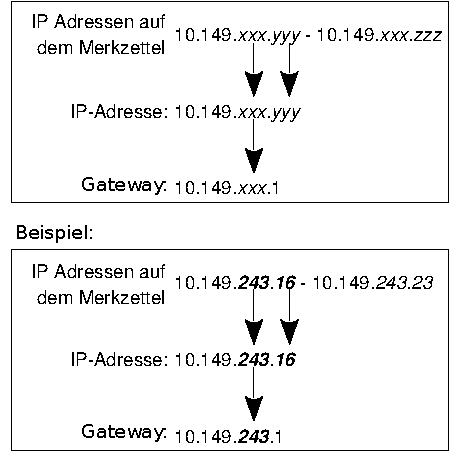
\includegraphics[width=\linewidth,keepaspectratio]{Bilder/IP_Gerneric}
		\end{minipage}
	\end{figure}

\pagebreak
%\enlargethispage{20pt}

\section{Einrichtungsanleitungen}
\label{section_netzweradresse}
\subsection{Router}

Jeder Router braucht leicht andere Einstellungen.
Auf dieser Seite haben wir Schlagworte gesammelt, um in der Anleitung die richtigen Abschnitte zu finden.

\url{https://stustanet.de/de/support/router_instructions/}

\subsection{Windows}

\begin{figure}[h]
	\raggedleft
	\vspace{-35pt}
	
\includegraphics[height=0.7cm,keepaspectratio]{Bilder/Windows_logo}
	\vspace{-25pt}
\end{figure}

\subsubsection*{Netzwerk Windows 10}

\begin{minipage}{0.6\textwidth}
\begin{enumerate}
	\item Klicken Sie auf das Windowssymbol in der unteren linken Ecke und anschließend auf \emph{Einstellungen}
	\item Klicken Sie auf \textit{Netzwerk und Internet}. Scrollen Sie runter bis \textit{Netzwerk und Freigabecenter} und klicken auf diesen Punkt. Wählen Sie in der linken Spalte den Punkt \textit{Adaptereinstellungen ändern}. Sollten Sie diesen Punkt nicht finden können Sie auch in der Suchzeile rechts oben nach \glqq Adaptereinstellungen ändern\grqq suchen.
%	\begin{figure}[h!]
%	\centering
%		\begin{minipage}[c]{0.3\linewidth}
%			\centering
%			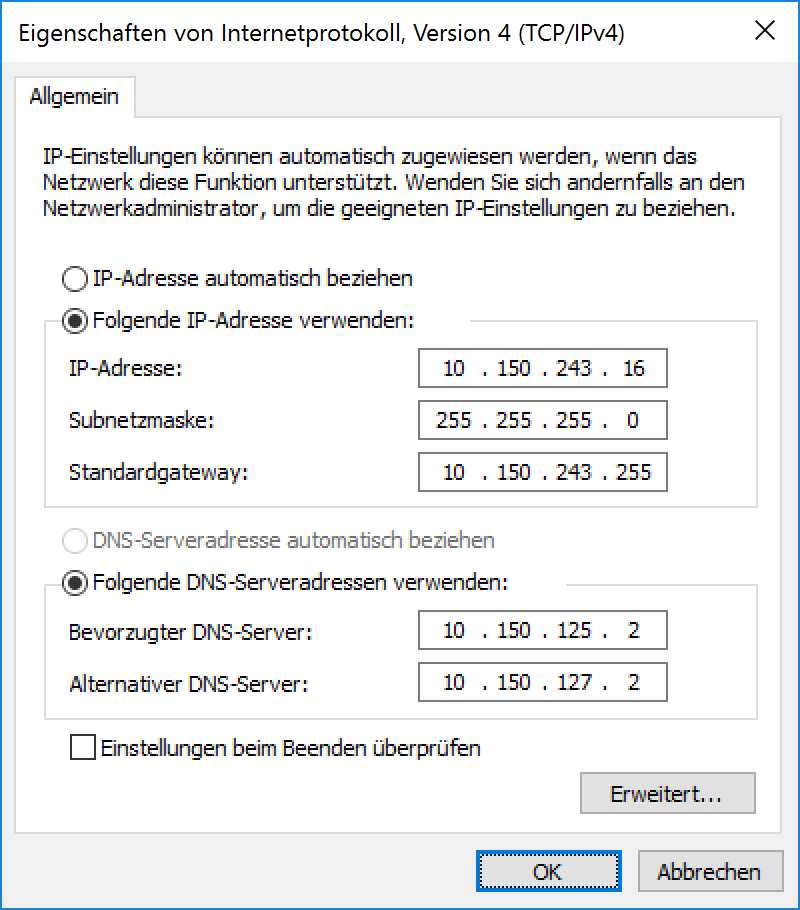
\includegraphics[width=0.9\linewidth,keepaspectratio]{Bilder/IP_Windows}
%			\caption{Beispielhafte Netzwerkeinstellungen unter Ubuntu Linux}
%			\vspace{-15pt}
%		\end{minipage}
%	\end{figure}

    \item Ihnen sollten nun mehrere Netzwerkverbindungen aufgelistet sein. Klicken Sie mit der \textbf{rechten} Maustaste auf \textit{Ethernet} und klicken Sie dann auf \textit{Eigenschaften}.
    \item Markieren Sie den Eintrag \textit{Internetprotokoll Version 4 (TCP/IPv4)} und klicken Sie danach auf Eigenschaften.
    \item Jetzt geben Sie IP-Adresse, Subnetzmaske/Subnetzpräfixlänge, Standardgateway und DNS Server ein.
    \item Klicken Sie auf Erweitert und wählen im folgenden Dialog den Reiter DNS aus. Tragen Sie im Feld DNS-Suffix für diese Verbindung \textbf{stusta.mhn.de} ein.
    \item Bestätigen mit OK.
\end{enumerate}
\end{minipage}
\begin{minipage}{0.4\textwidth}
	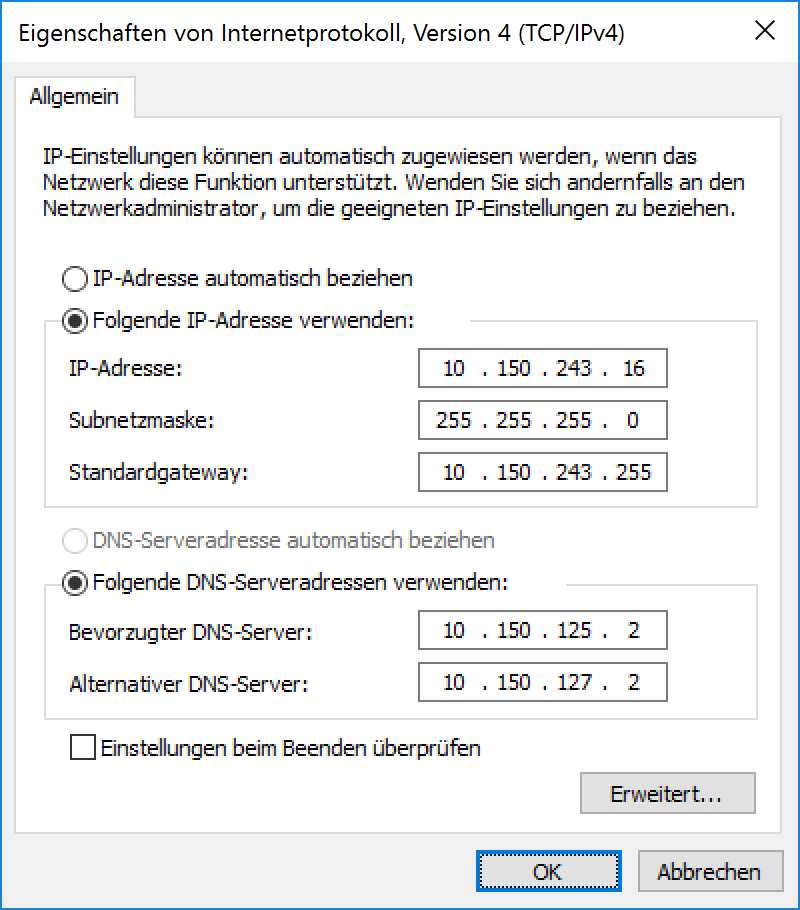
\includegraphics[width=\linewidth]{Bilder/IP_Windows}
	%  \caption{Bildunterschrift}
\end{minipage}

\subsubsection*{Netzwerk Windows 11}
\begin{minipage}{0.6\textwidth}
\begin{enumerate}
	\item Gehe zu \textit{Einstellungen} $\rightarrow$ \textit{Netzwerk und Internet} $\rightarrow$ \textit{Ethernet} $\rightarrow$ Bei \textit{IP-Zuweisung} klicke \textit{Bearbeiten}
	\item Ändere das Drop-Down-Menü zu \textit{Manuell}
	\item Setze \textit{IPv4} auf \textit{Ein}
	\item Jetzt trage
		\subitem IP-Adresse
		\subitem Subnetzmaske
		\subitem Gateway
		\subitem Bevorzugter DNS
		\subitem Alternativer DNS \\
	deines Zimmers ein.
	\item Bestätige mit Speichern.
\end{enumerate}
\end{minipage}
\begin{minipage}{0.4\textwidth}
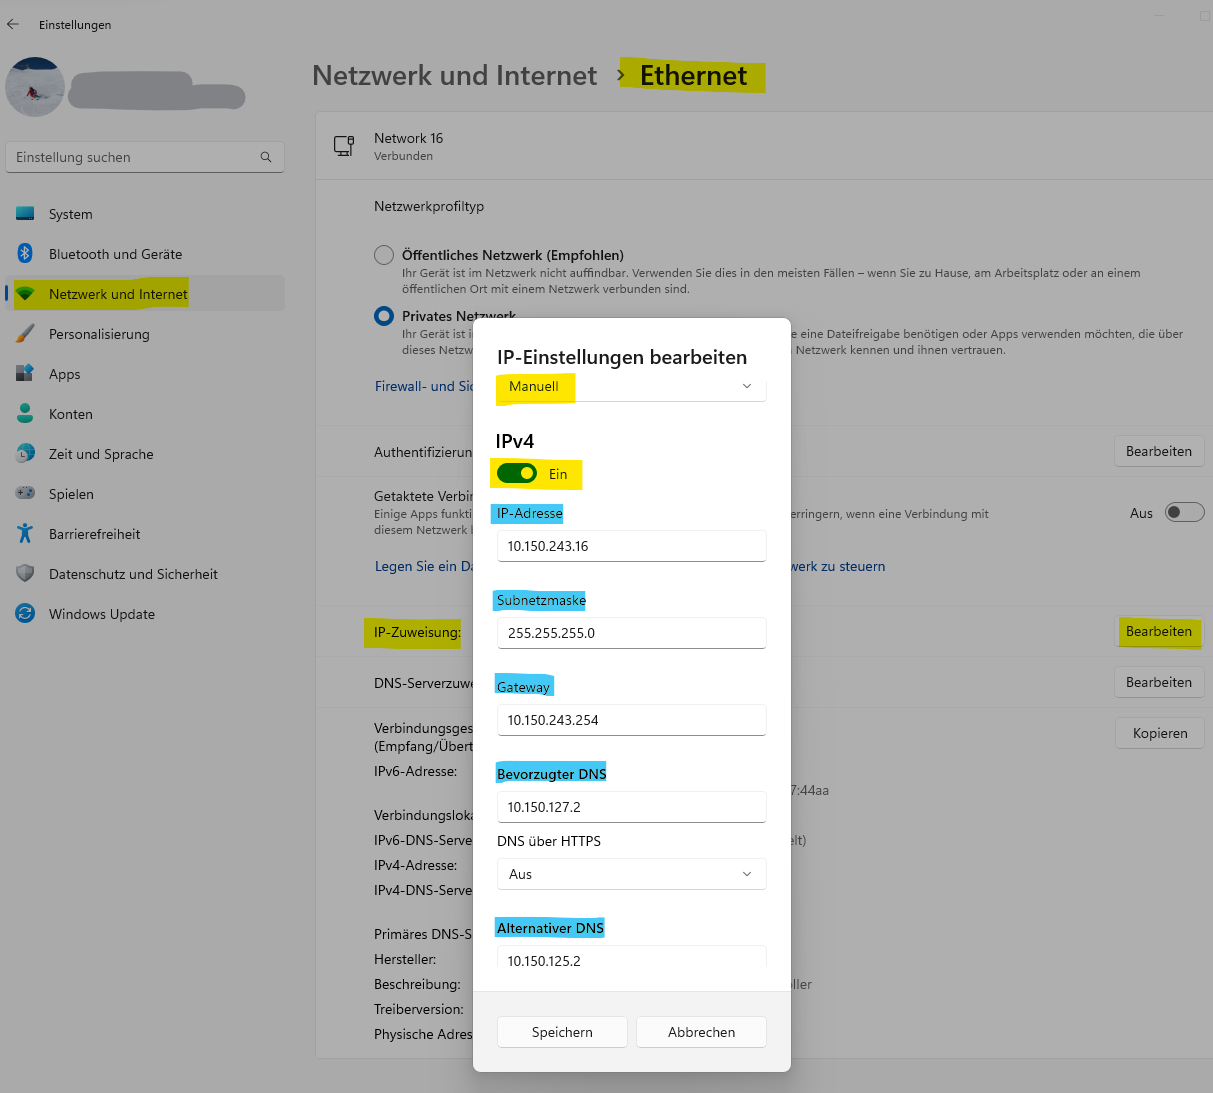
\includegraphics[width=\linewidth]{Bilder/Win11/ip_win11_de}
\end{minipage}

\subsubsection*{Globaler Proxy Win 10/11}

\begin{enumerate}
	\item Wähle \textit{Einstellungen} $\rightarrow$ \textit{Netzwerk und Internet} $\rightarrow$ \textit{Proxy}
	
	%	\item Deaktivieren Sie die Option \emph{Einstellungen automatisch erkennen}.
	
	\subitem \textbf{Nur Windows 11:} Klicke bei \textit{Setupskript verwenden} auf den Button  \textit{Einrichten}
	
	\setcounter{enumi}{1}
	\item Setze \textit{Setupskript verwenden} auf \textit{Ein}
	\item Trage als Skriptadresse die \textit{.pac Proxyskript-Adresse} deines Zimmers ein.
	\item Bestätige mit Speichern
\end{enumerate}

\begin{figure}[h]
	\centering
	\begin{minipage}{.55\textwidth}
		\centering
		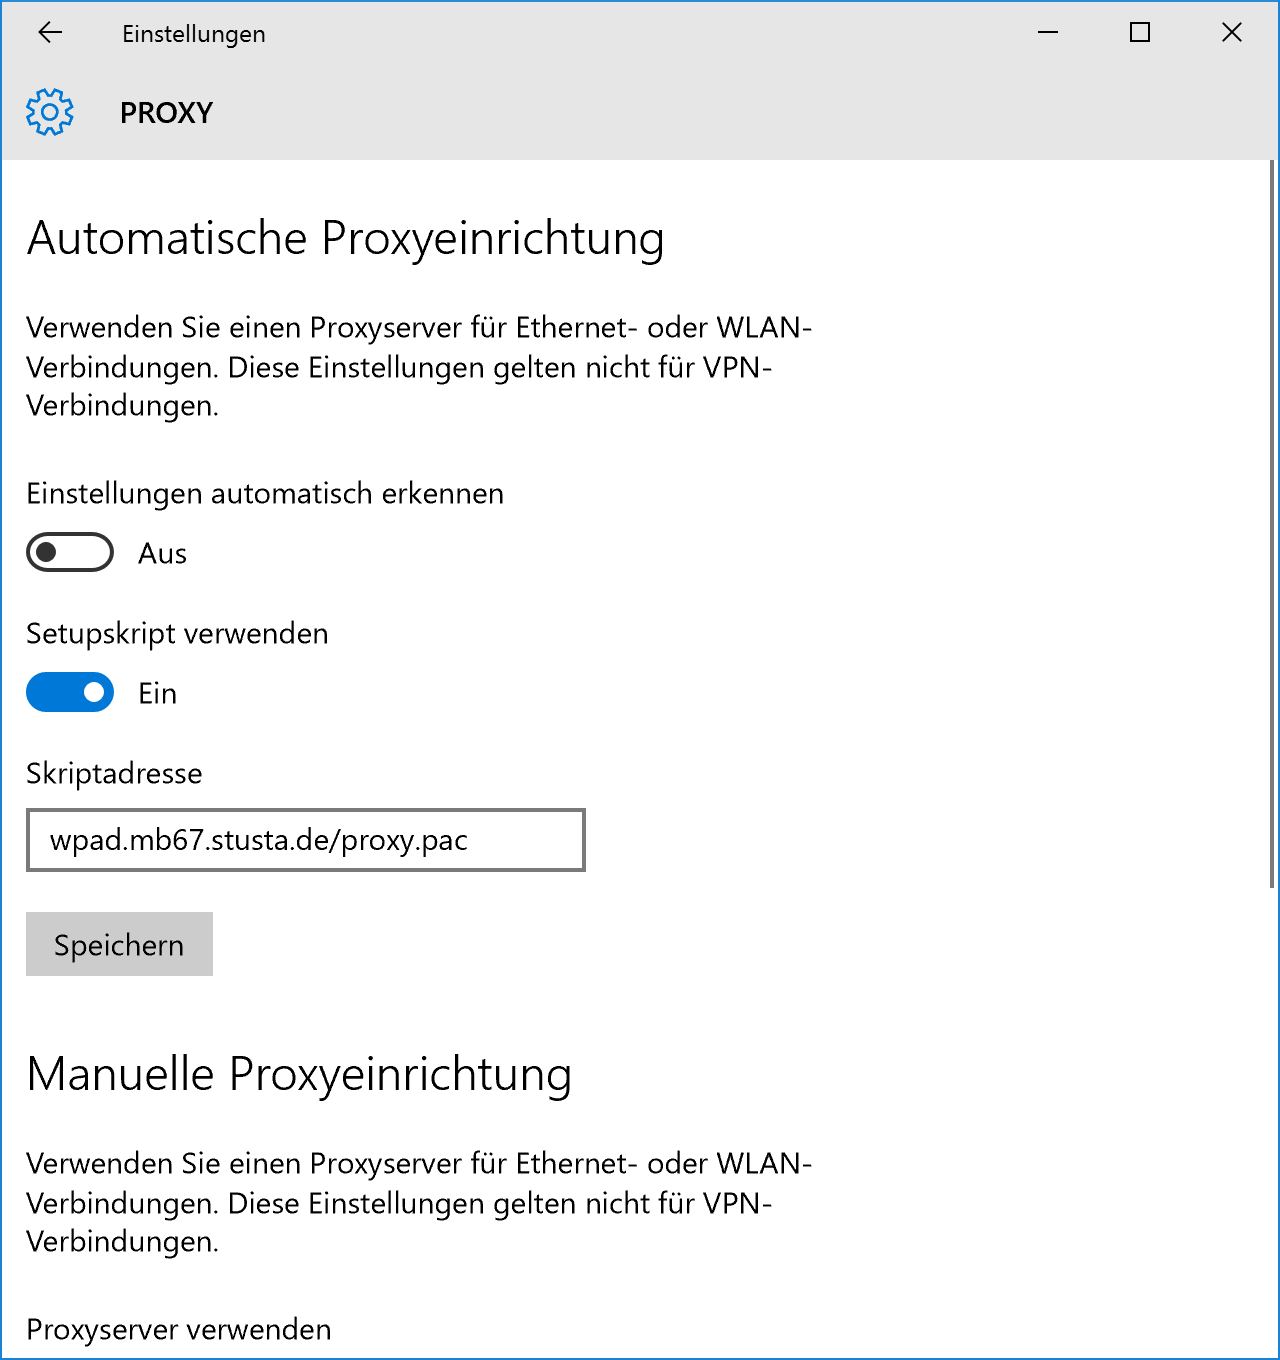
\includegraphics[height=.20\textheight]{Bilder/Proxy_Edge}
	\end{minipage}
	\begin{minipage}{.30\textwidth}
		\centering
		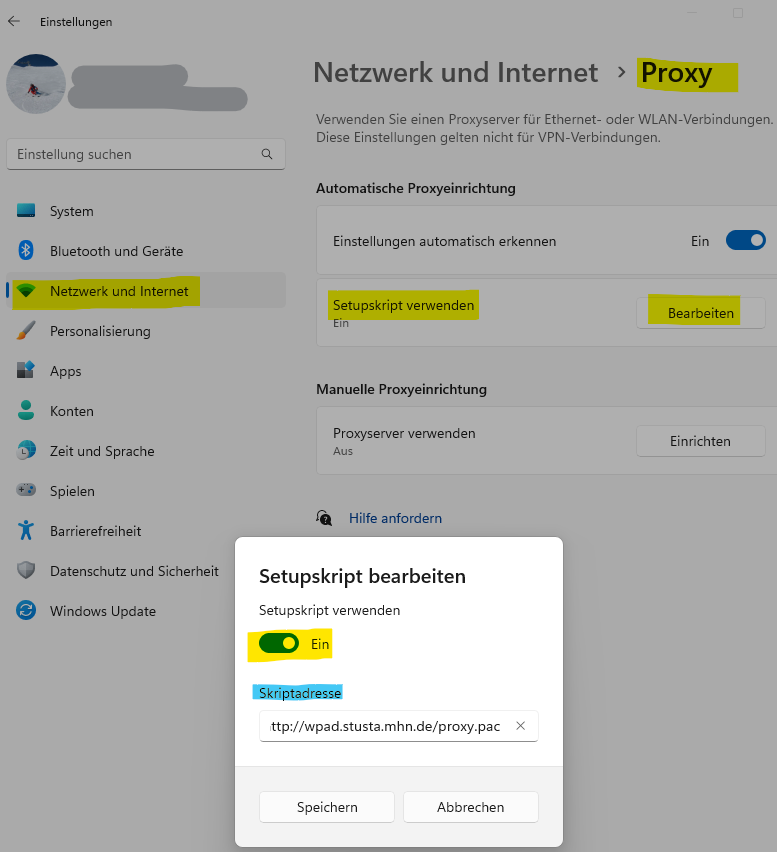
\includegraphics[height=.20\textheight]{Bilder/Win11/proxy_win11_de}
	\end{minipage}
\end{figure}

\pagebreak

\subsection{Linux}

\subsubsection*{Netzwerkeinstellungen}

\begin{figure}[h]
	\raggedleft
	\vspace{-35pt}
	
\includegraphics[height=0.7cm,keepaspectratio]{Bilder/linux_logo_neu}
	\vspace{-20pt}
\end{figure}

\begin{minipage}{0.6\textwidth}
\begin{enumerate}
	\item Öffnen Sie die Netzwerkkonfiguration durch Klick auf \emph{System} $\rightarrow$ \emph{Einstellungen} $\rightarrow$ \emph{Netzwerkkonfiguration}.
	\item Markieren Sie nun im Reiter Kabelgebunden den entsprechenden Eintrag Ihrer Netzwerkkarte (im Normalfall \emph{eth0}) und klicken Sie auf den Button \emph{Bearbeiten}.
	\item Gehen Sie zum Reiter \emph{IPv4-Einstellungen} und setzen Sie Methode auf \emph{Manuell}.
	\item Unter \emph{Adressen} klicken Sie auf den Button \emph{Hinzufügen}.
	\item Jetzt geben Sie IP-Adresse, Subnetzmaske, Gateway, DNS und Suchdomäne ein. Die Adressen der DNS-Server lauten \textbf{10.150.127.2} und \textbf{10.150.125.2}, die Suchdomäne \textbf{stusta.mhn.de} und die Netzmaske \textbf{255.255.255.0}. Ihre jeweilige IP-Adresse steht auf einem Aufkleber auf Ihrer Anschlussbuchse bzw. auf dem Zettel, den Sie mit Ihrem Mietvertrag erhalten haben. Sollten Sie einen neuen Zettel benötigen, wenden Sie sich bitte an die Hausverwaltung oder besuchen Sie unsere Sprechstunde. Bestätigen Sie mit \emph{OK} und schließen Sie das Fenster für die Netzwerkeinstellungen.
\end{enumerate}
\end{minipage}
\begin{minipage}{0.4\textwidth}
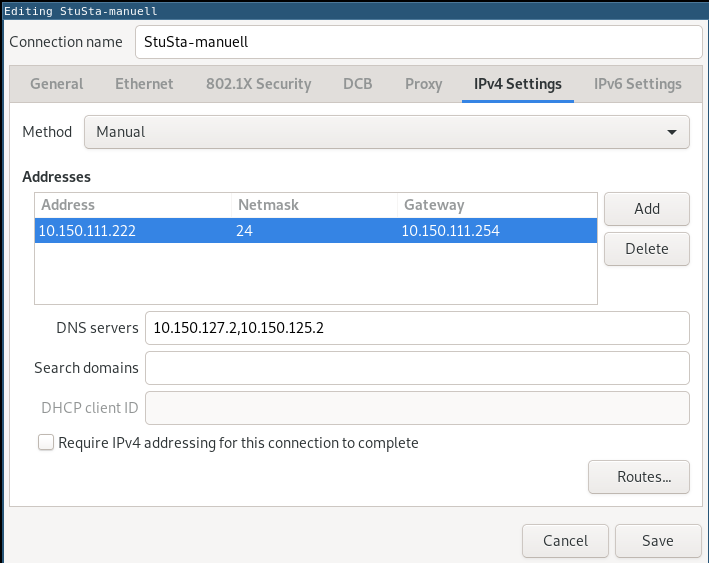
\includegraphics[width=\linewidth]{Bilder/IP_Ubuntu_neu}
%  \caption{Bildunterschrift}
\end{minipage}

\subsubsection*{Globaler Proxy}

\begin{enumerate}
	\item Öffnen Sie die Netzwerk-Proxy-Einstellungen durch Klick auf \emph{System} $\rightarrow$ \emph{Einstellungen} $\rightarrow$ \emph{Netzwerk-Proxy}.
	\item Hier markieren Sie ganz unten die Option \emph{Automatische Proxy-Konfiguration} und tragen bei URL für Auto-Konfiguration: \url{http://wpad.stusta.mhn.de/proxy.pac} ein. Schließen Sie das Fenster. 
\end{enumerate}

\pagebreak

\subsection{MacOS}

\begin{figure}[h]
	\raggedleft
	\vspace{-35pt}
	
\includegraphics[height=0.7cm,keepaspectratio]{Bilder/apple_logo_neu}
	\vspace{-20pt}
\end{figure}

\subsubsection*{Netzwerkeinstellungen}

\begin{minipage}{0.6\textwidth}
\begin{enumerate}
    \item Öffnen Sie die Netzwerkkonfiguration durch Klick auf \emph{Apfel} (oben links) und wählen dann \emph{Systemeinstellungen} $\rightarrow$ \emph{Netzwerk} aus.
    \item Markieren Sie nun das Netzwerkgerät \emph{Ethernet}.
    \item Setzen Sie das Feld \emph{IPv4 Konfigurieren} auf \emph{Manuell}.
    \item Jetzt geben Sie IP-Adresse, Teilnetzmaske, Gateway, DNS-Server und Such-Domains ein. Die Adressen der DNS-Server lauten \textbf{10.150.127.2} und \textbf{10.150.125.2}, die Such-Domains \textbf{stusta.mhn.de} und die Teilnetzmaske \textbf{255.255.255.0}. Ihre jeweilige IP-Adresse steht auf einem Aufkleber auf Ihrer Anschlussbuchse bzw. auf dem Internetkonfigurationsblatt, das Sie mit Ihrem Mietvertrag erhalten haben. Sollten Sie dieses Blatt nicht mehr finden, wenden Sie sich bitte an die Hausverwaltung oder besuchen Sie unsere Sprechstunde.
    Bestätigen Sie mit \emph{Anwenden}.
\end{enumerate}
\end{minipage}
\begin{minipage}{0.4\textwidth}
	\centering
	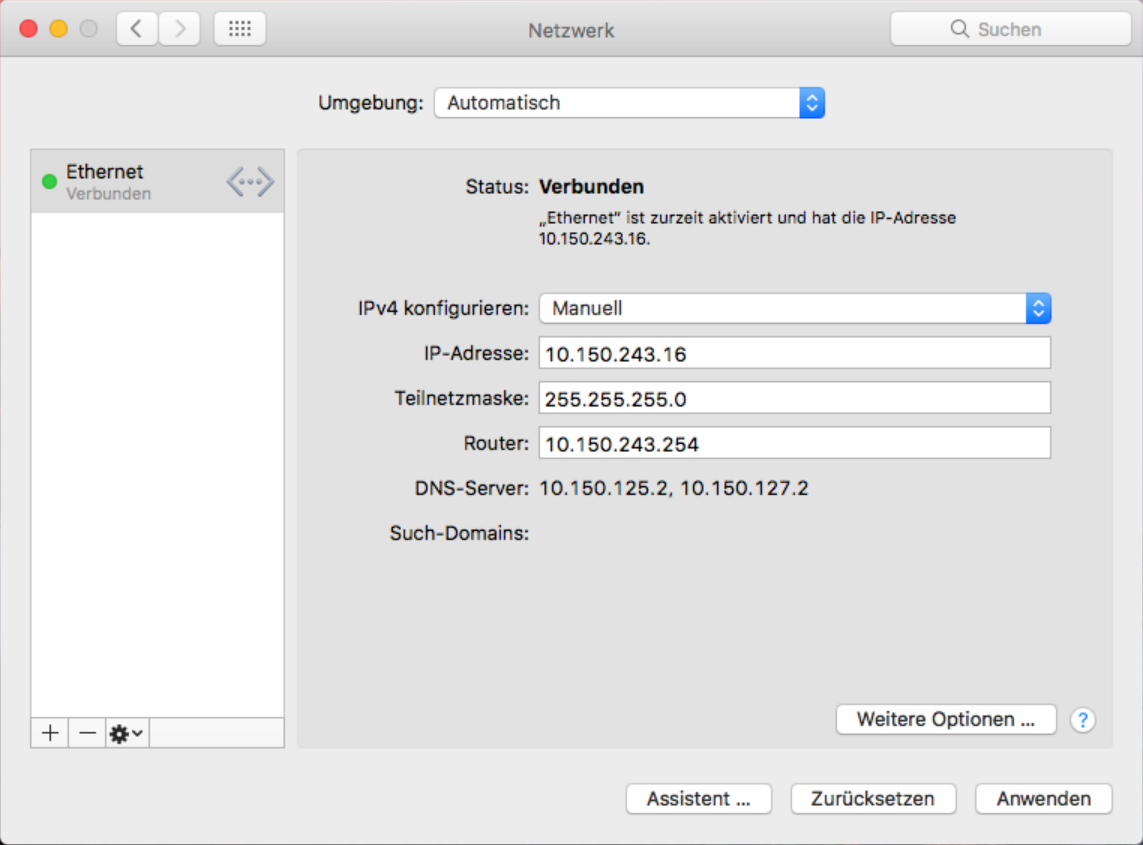
\includegraphics[width=\linewidth,keepaspectratio]{Bilder/IP_MAC}
\end{minipage}

\subsubsection*{Globaler Proxy}

\begin{enumerate}
	\item Öffnen Sie mit dem Button \emph{Weitere Optionen...} im voherigen Dialog die Detaileinstellungen und wechseln sie auf die Registerkarte \emph{Proxies}
	\item Setzen sie bei Zu konfigurierendes Protokoll vor Autom. Proxy-Konfiguration einen Hacken und tragen rechts bei URL \url{http://wpad.stusta.mhn.de/proxy.pac} ein. Schließen Sie die Detaileinstellungen mit OK und bestätigen Sie erneut mit Anwenden. Sie können die Netzwerkeinstellungen jetzt schließen.
\end{enumerate}

\subsection{Globaler Proxy Android}
Bei den verschiedenen Herstellern kann das Interface leider abweichen.
Wenn du Probleme hast, kann du versuchen im Internet nach Anleitungen für dein Handymodell in Verbindung mit den Schlagworten \textit{Proxy Einrichtung} suchen.

\subsubsection*{Google Pixel Android 12}
\begin{enumerate}
	\item Öffne die WLAN-Einstellungen
	\item Klicke auf das Zahnrad neben dem Namen deines WLAN-Netzwerkes
	\item Klicke auf das Stiftsymbol am oberen rechten Bildschirmrand
	\item Aktiviere das Drop-Down-Menü \textit{Erweiterte Optionen}
	\item Wähle unter \textit{Proxy} den Punkt \textit{Automatische Proxykonfiguration}
	\item Trage als \textit{PAC-URL} die \textit{.pac Proxyskript-Adresse} deines Zimmers ein.
	\item Bestätige mit Speichern
\end{enumerate}

\begin{figure}[h]
	\centering
	\begin{minipage}{0.20\textwidth}
		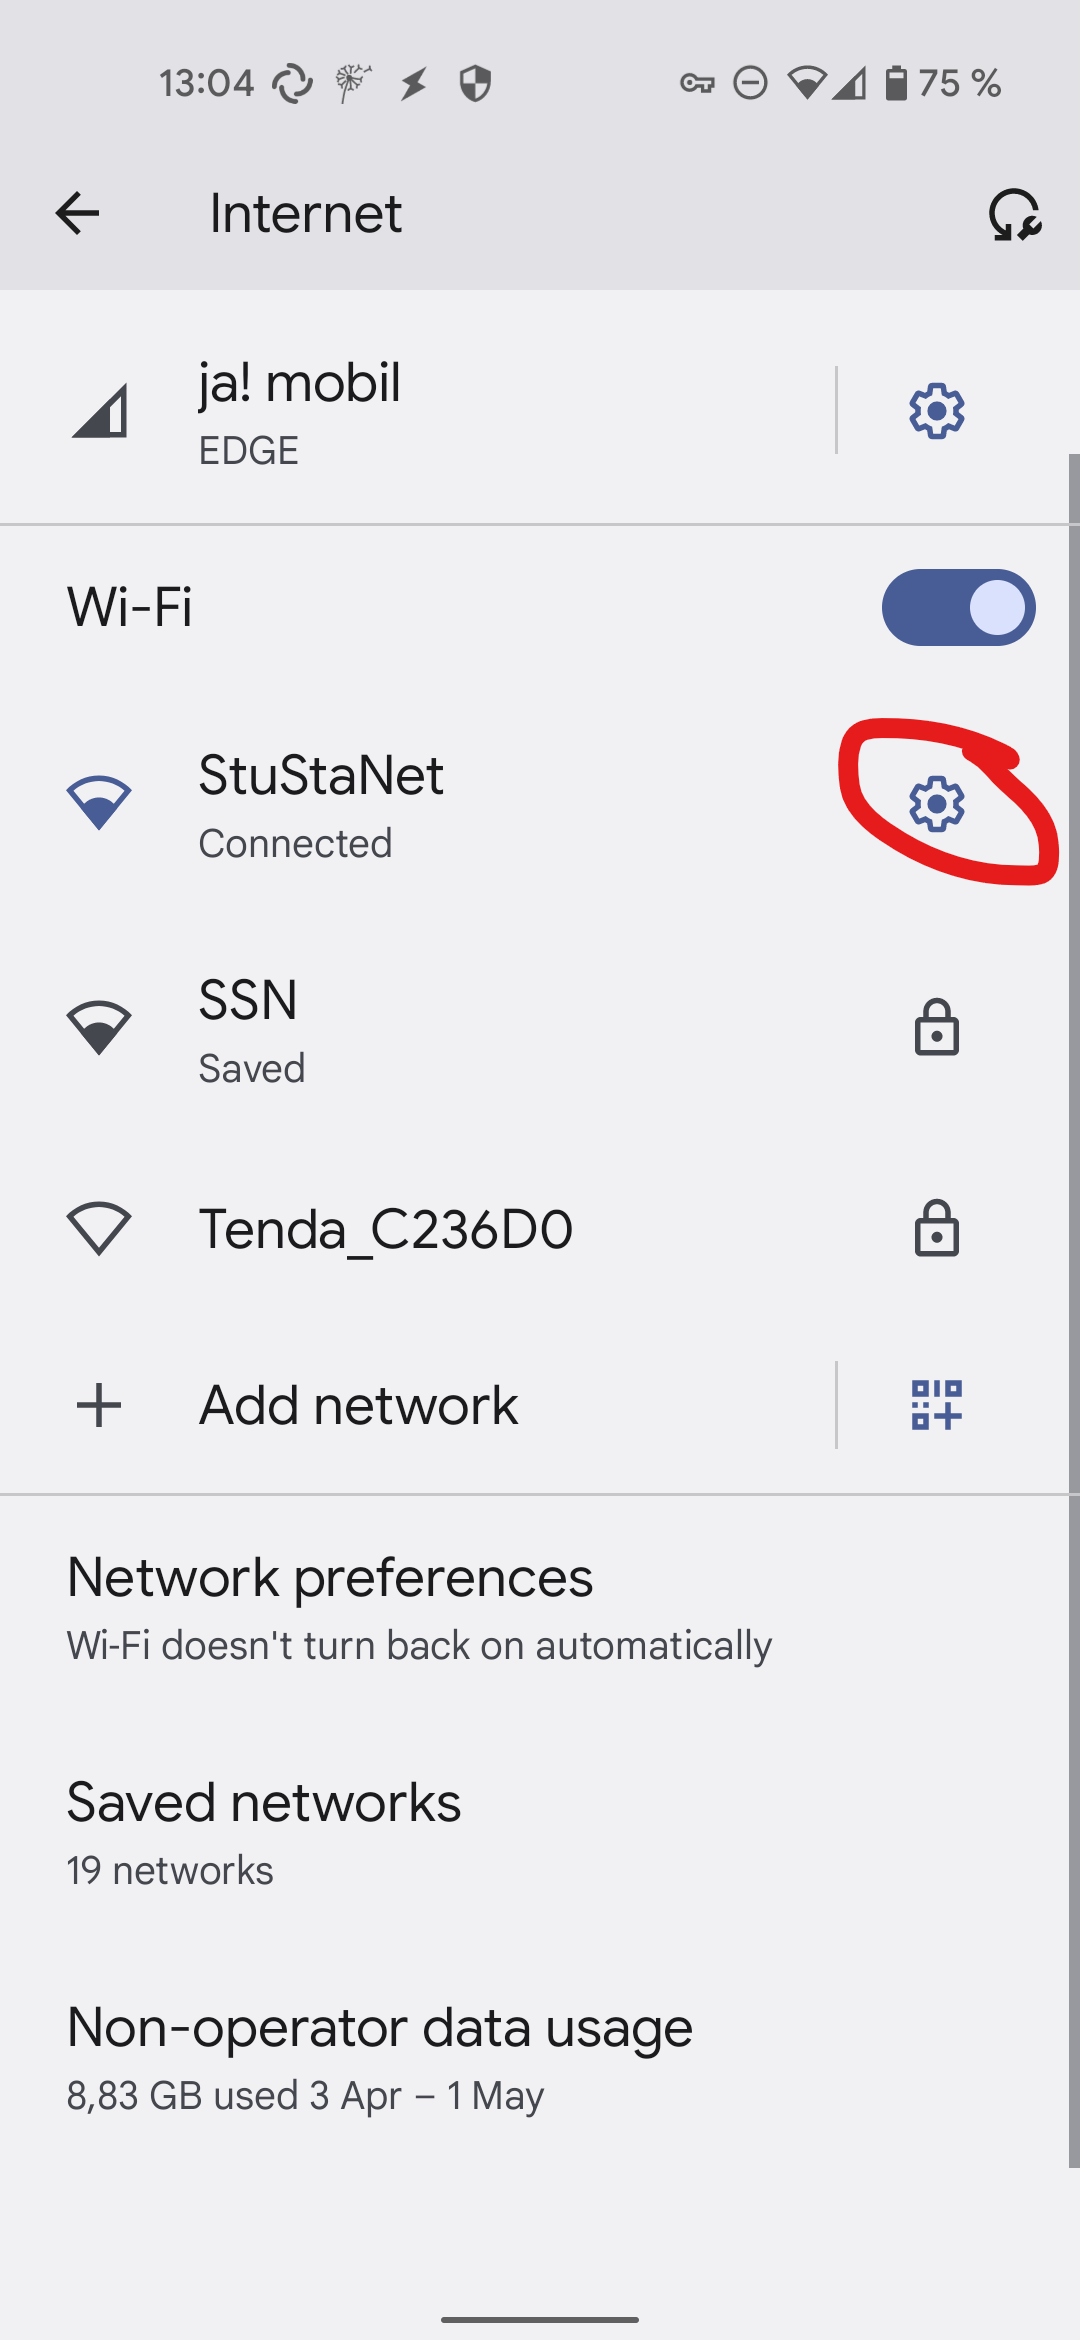
\includegraphics[width=0.7\linewidth,keepaspectratio]{Bilder/Android/android12_1}
	\end{minipage}
	\begin{minipage}{0.20\textwidth}
		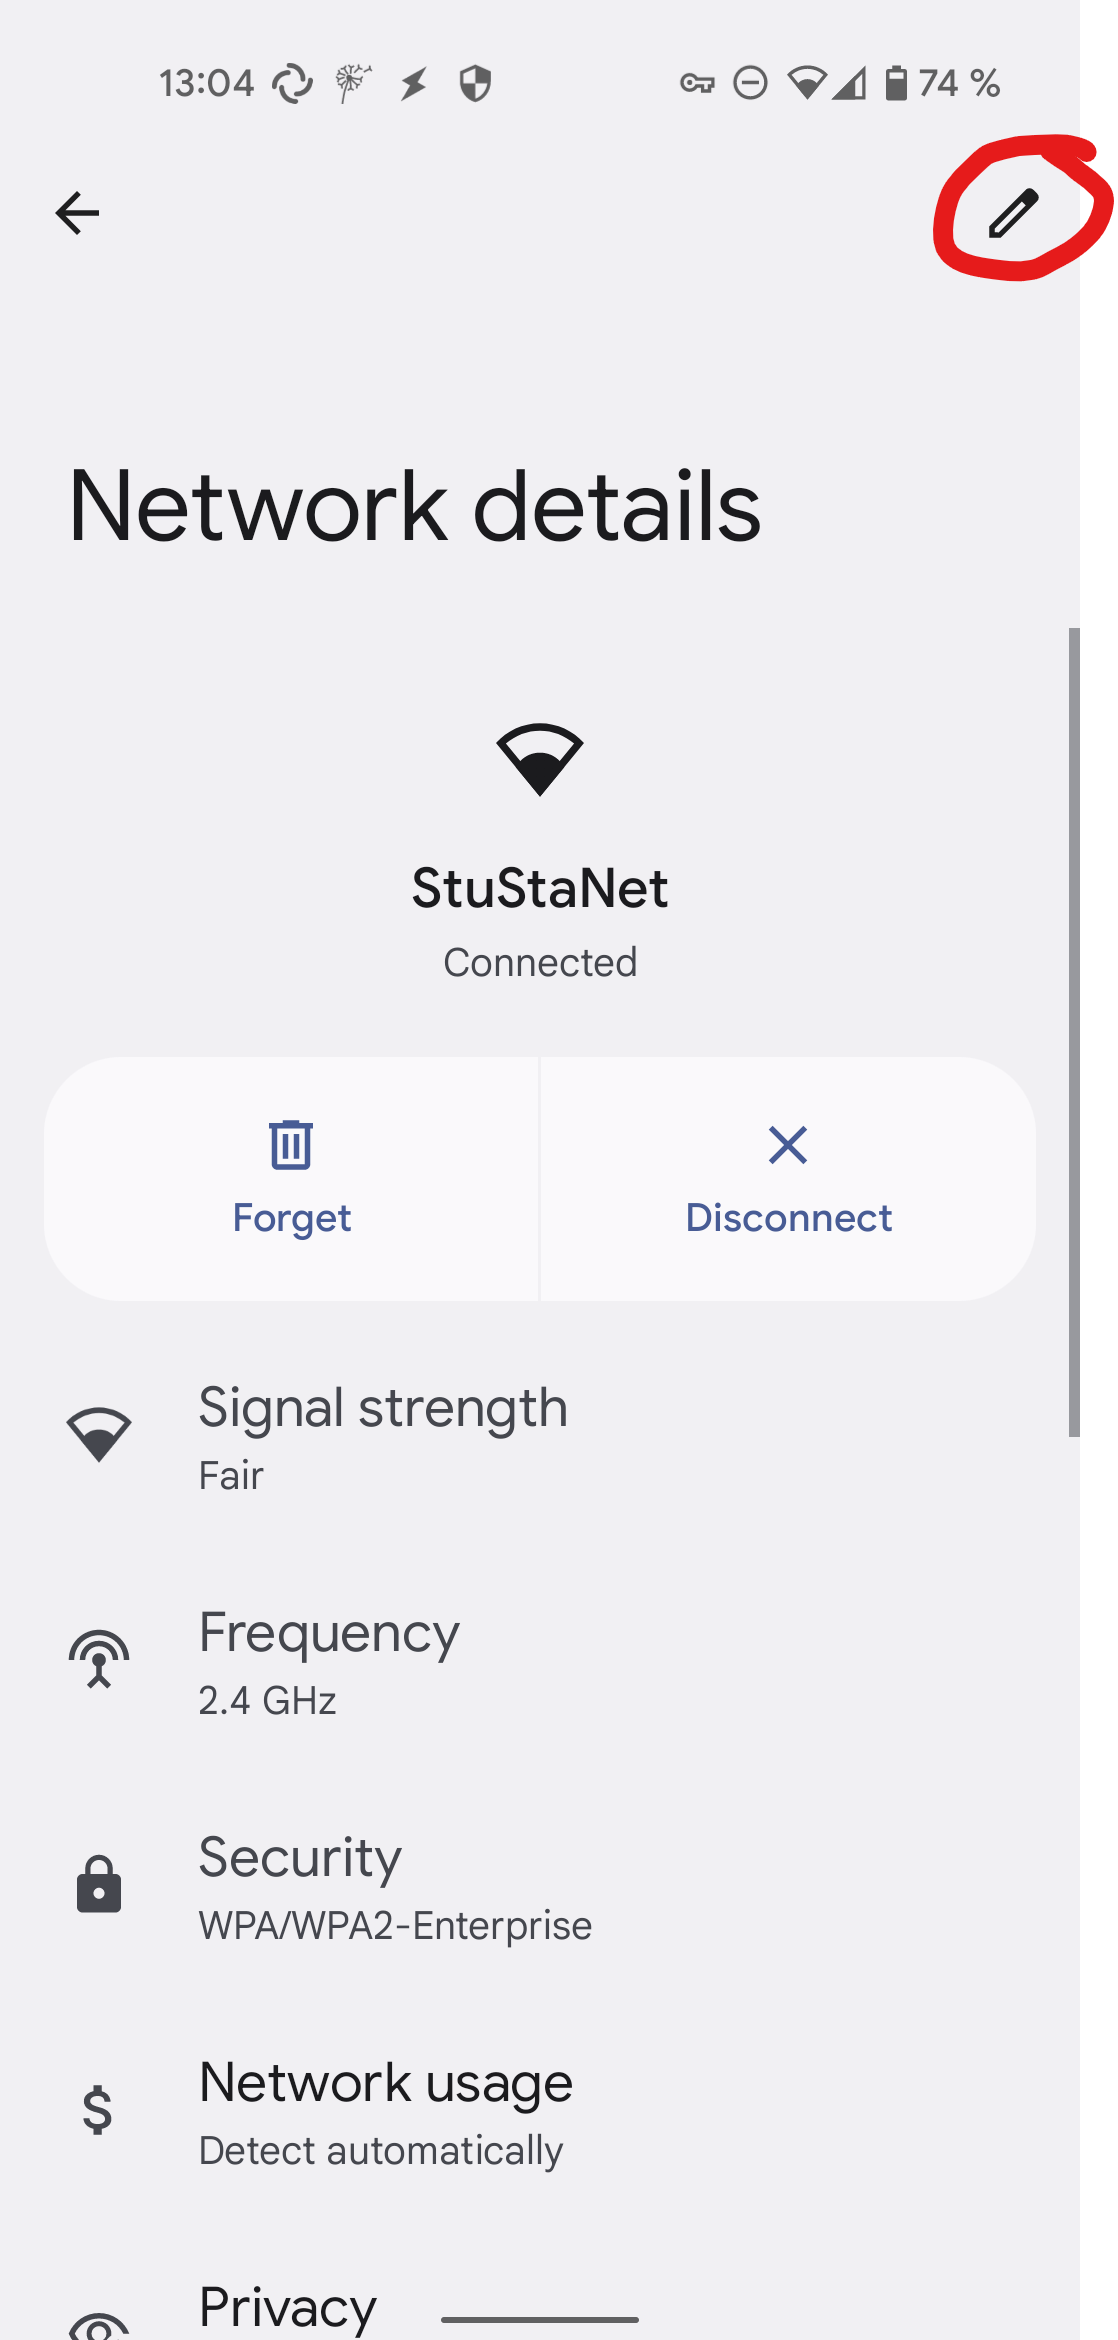
\includegraphics[width=0.7\linewidth,keepaspectratio]{Bilder/Android/android12_2}
	\end{minipage}
	\begin{minipage}{0.20\textwidth}
		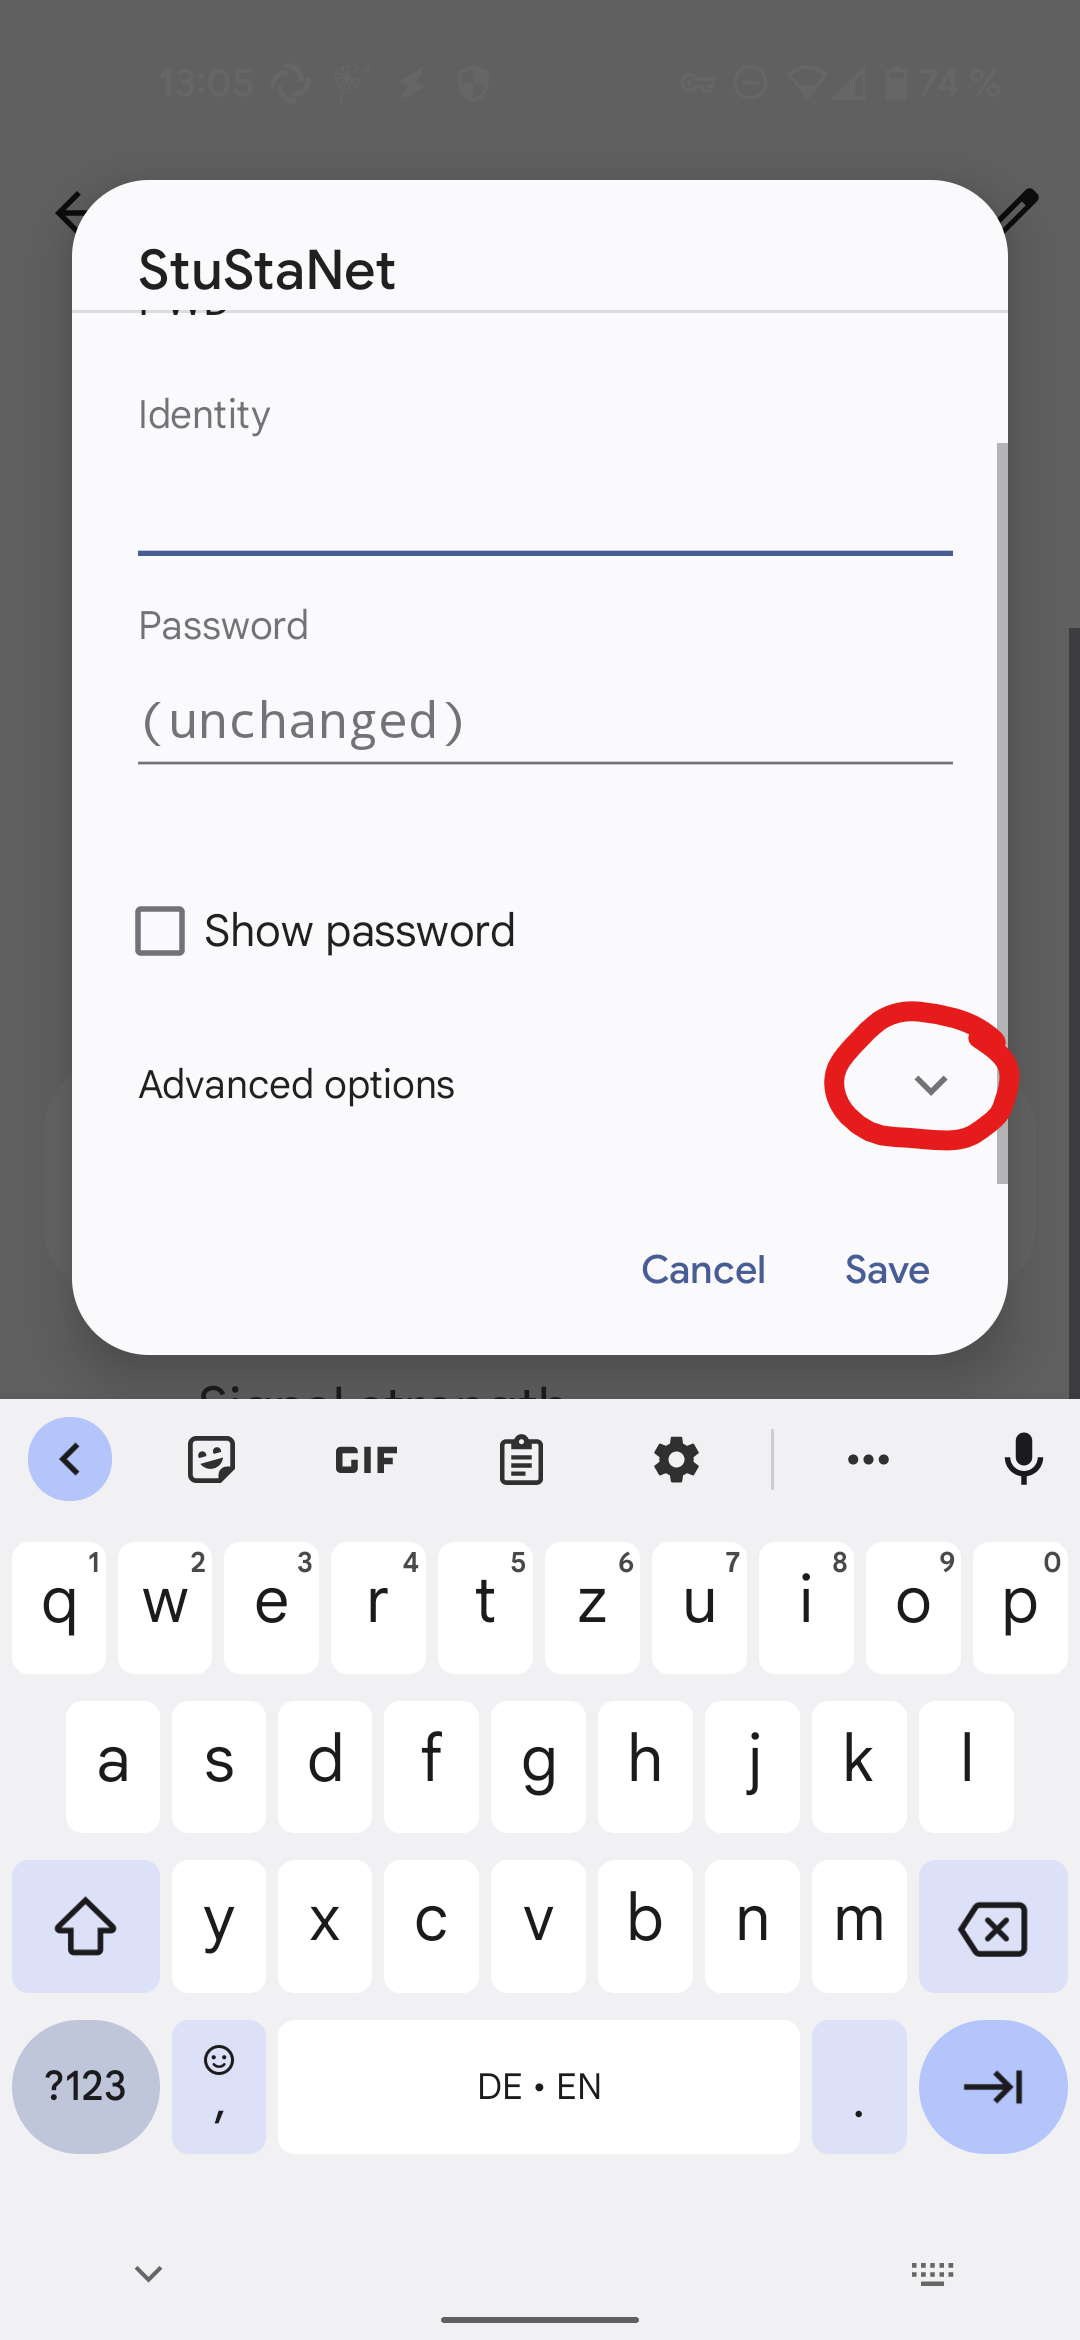
\includegraphics[width=0.7\linewidth,keepaspectratio]{Bilder/Android/android12_3}
	\end{minipage}
	\begin{minipage}{0.20\textwidth}
		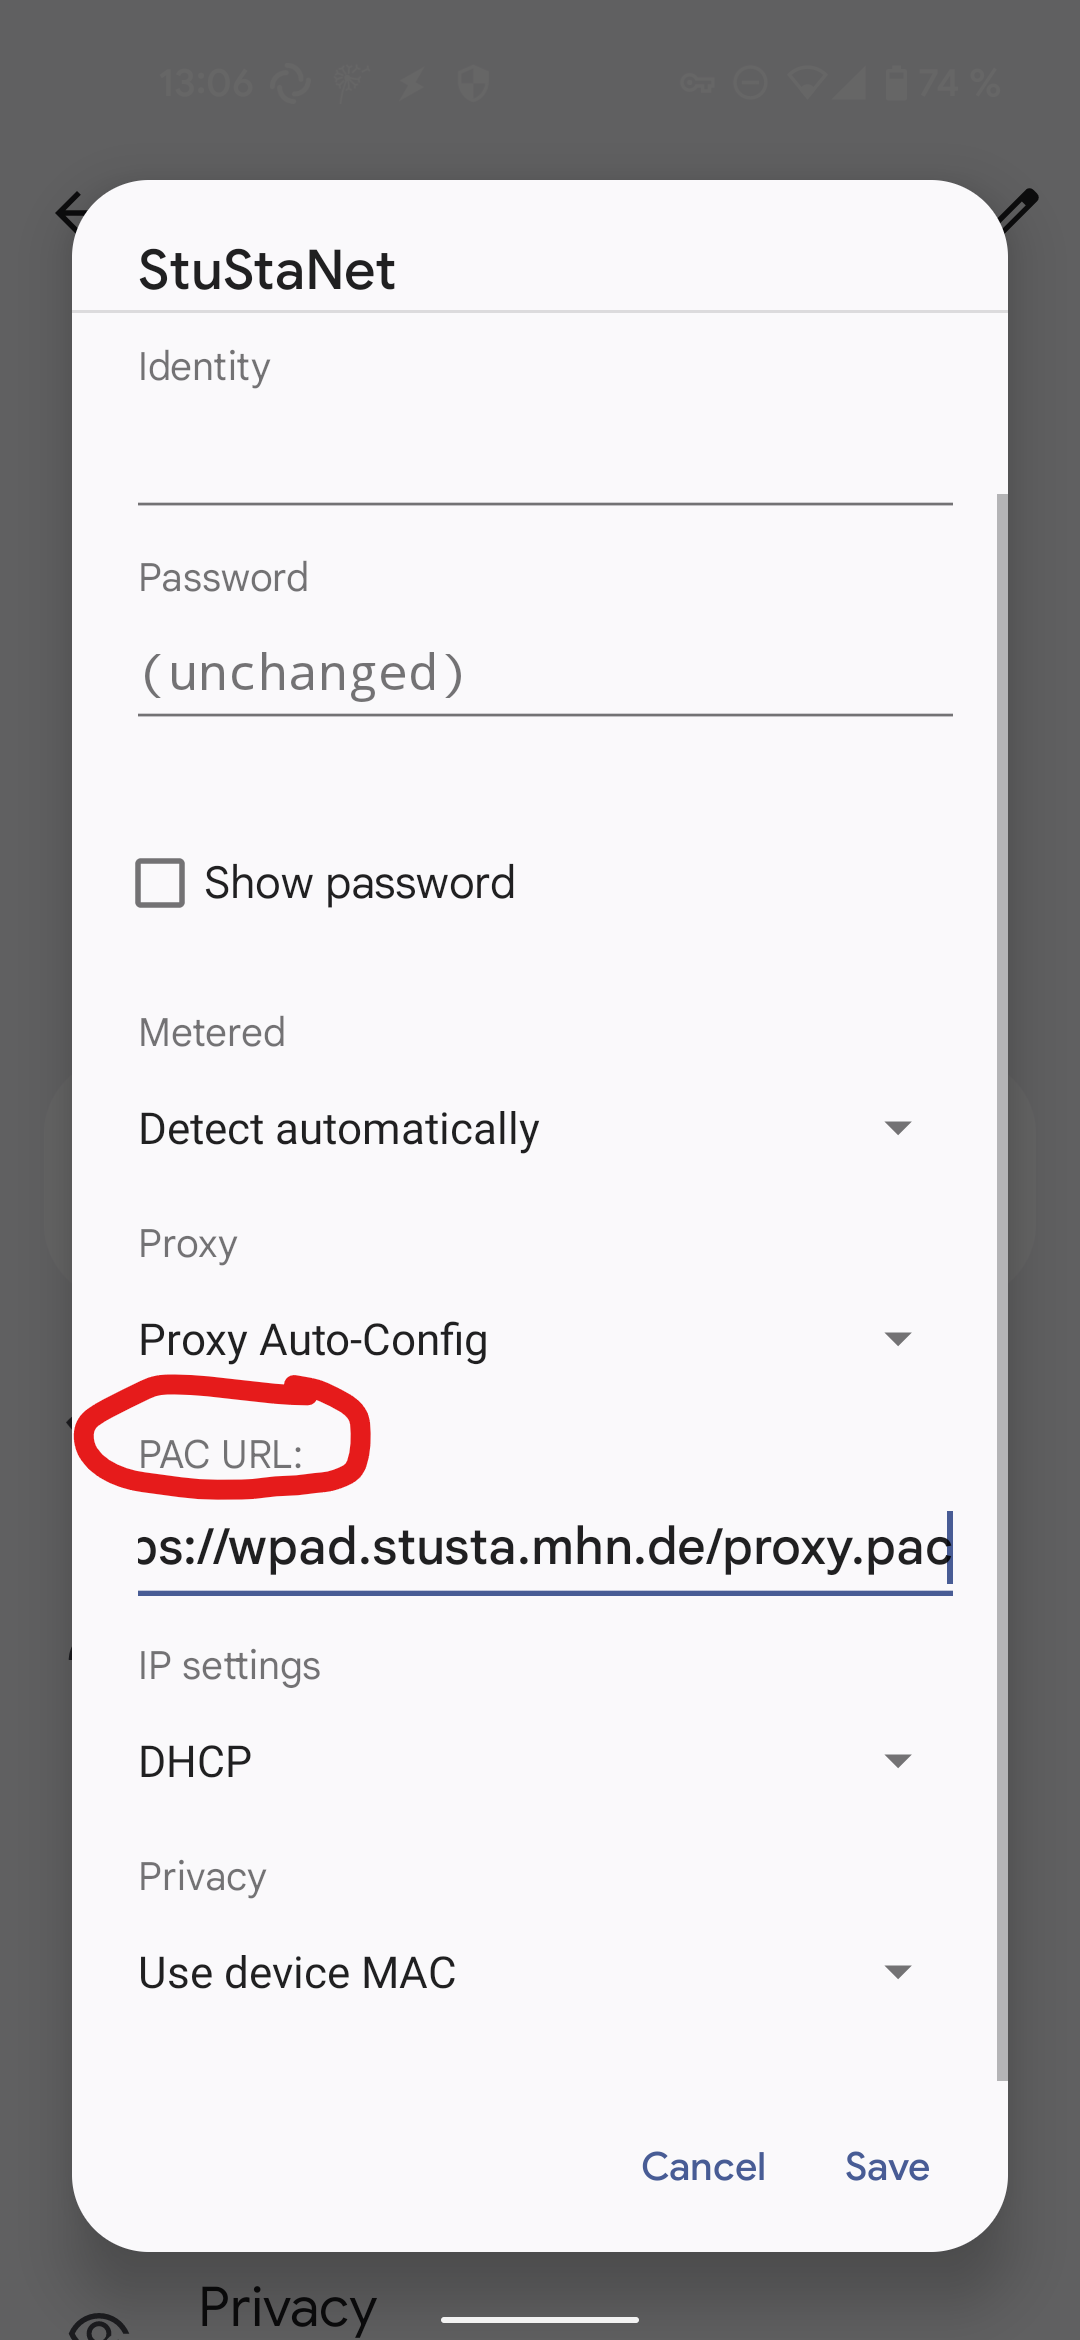
\includegraphics[width=0.7\linewidth,keepaspectratio]{Bilder/Android/android12_4}
	\end{minipage}
\end{figure}

\subsection{Globaler Proxy andere Geräte}

Wenn du Probleme hast, kann du versuchen im Internet nach Anleitungen für dein Gerät in Verbindung mit den Schlagworten \textit{Proxy Einrichtung} suchen.

\subsection{Proxy-Konfiguration im Browser (nur Nicht-Mitglieder)}
\label{Proxy}

\subsubsection*{Mozilla Firefox}

\begin{figure}[h]
	\raggedleft
	\vspace{-25pt}
	
\includegraphics[height=0.7cm,keepaspectratio]{Bilder/Firefox_35_logo}
	\vspace{-20pt}
\end{figure}

\begin{minipage}{0.6\textwidth}
\begin{enumerate}
	\item Klicken Sie auf die 3 übereinanderliegenden Striche in der rechten oberen Ecke, wählen Sie danach \emph{Einstellungen}.
	\item Gehen Sie zum Punkt \emph{Verbindungs-Einstellungen} und wählen diesen aus.
	\item Markieren Sie den Punkt \emph{Automatische Proxy-Konfigurations-Adresse} und tragen Sie als automatische Proxy-Konfigurations-URL: \\ \url{http://wpad.stusta.mhn.de/proxy.pac} ein.
	\item Bestätigen Sie mit OK .
\end{enumerate}
\end{minipage}
\begin{minipage}{0.4\textwidth}
\centering
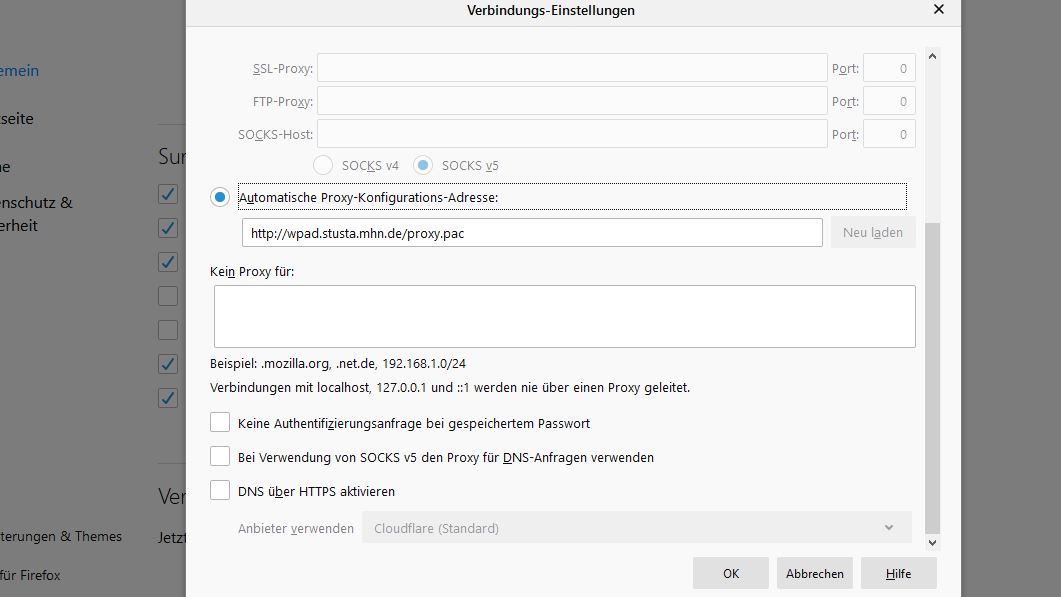
\includegraphics[width=\linewidth,keepaspectratio]{Bilder/Firefox_neu_proxy}
\end{minipage}


\subsubsection*{Google Chrome/Microsoft Edge}

Diese Browser verwenden die Proxyeinstellungen des Systems.
Sieh dir dafür den passenden Abschnitt weiter oben an.

\end{document}
